\input{preamble}

\section*{Muon decay}
From the Particle Data Group website\footnote{https://pdg.lbl.gov/2020/listings/rpp2020-list-muon.pdf}
%
\begin{center}
\begin{tikzpicture}
\node at (0,0) {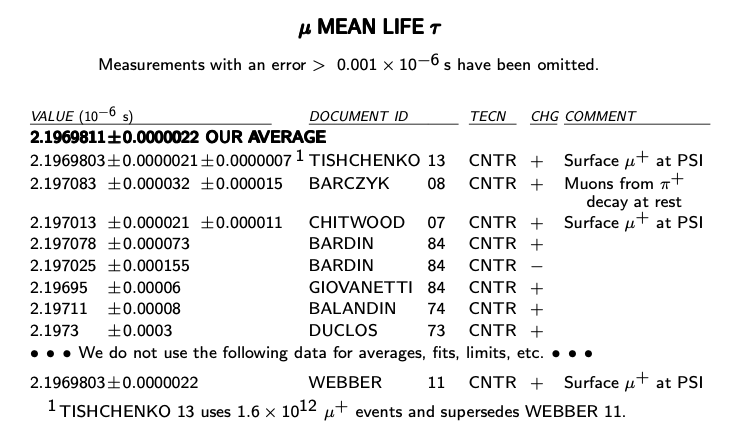
\includegraphics[scale=0.5]{muon-mean-life.png}};
\draw[red,very thick] (-6,2) rectangle (-0.6,1);
\end{tikzpicture}
\end{center}

From ``V minus A'' theory we have the following formula for muon lifetime $\tau$.
\begin{equation*}
\tau=\frac{96\pi^2h}{G_F^2\left(m_\mu c^2\right)^5}
\end{equation*}

Symbol $G_F$ is Fermi coupling constant, $m_\mu$ is muon mass.

\bigskip
From NIST we have
\begin{align*}
G_F&=1.1663787\times10^{-5}\;\text{GeV}^{-2}
\\
m_\mu&=1.883531627\times10^{-28}\;\text{kilogram}
\\
h&=6.62607015\times10^{-34}\;\text{joule}\;\text{second}\;\text{(exact)}
\\
c&=299792458\;\text{meter}\;\text{second}^{-1}\;\text{(exact)}
\\
1\,\text{eV}&=1.602176634\times10^{-19}\;\text{joule}\;\text{(exact)}
\end{align*}

Hence
\begin{equation*}
\tau=\frac{96\pi^2h}{G_F^2\left(m_\mu c^2\right)^5}
=2.18735\times10^{-6}\,\text{second}
\end{equation*}

The result is a bit smaller than the observed value from Particle Data Group.
\begin{equation*}
\frac{\tau}{\text{observed value}}
=\frac{2.18735\times10^{-6}\,\text{second}}{2.19698\times10^{-6}\;\text{second}}=0.9956
\end{equation*}

As the following diagram shows, a muon decays into a muon neutrino, an electron anti-neutrino,
and an electron.
\begin{center}
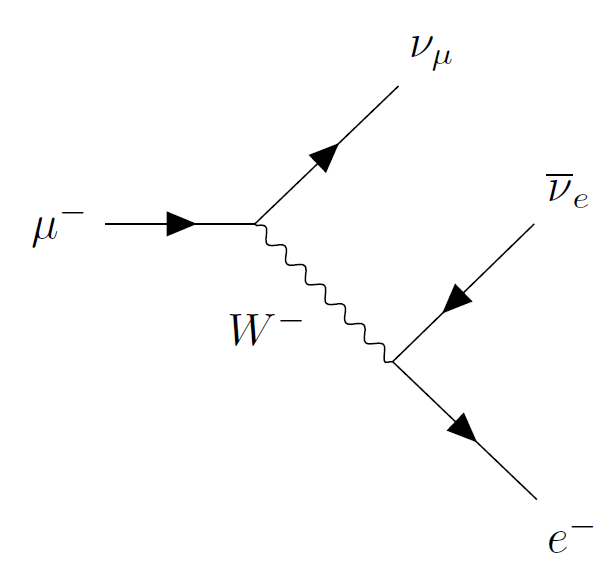
\includegraphics[scale=0.25]{muon-decay-diagram.png}
\end{center}

\begin{center}
\begin{tabular}{lcccc}
Particle & Momentum & Mass & Spin up & Spin down
\\[2ex]
Muon $\mu^-$ & $p_1$ & $m_1$ & $u_{11}$ & $u_{12}$
\\
Muon neutrino $\nu_\mu$ & $p_2$ & $m_2$ & $u_{21}$ & $u_{22}$
\\
Electron anti-neutrino $\bar{\nu}_e$ & $p_3$ & $m_3$ & $v_{31}$ & $v_{32}$
\\
Electron $e^-$ & $p_4$ & $m_4$ & $u_{41}$ & $u_{42}$
\end{tabular}
\end{center}

For $E_n=\sqrt{{\mathbf p_n}^2+{m_n}^2}$ we have
\begin{equation*}
p_1=\underset{\mu^-}
{\begin{pmatrix}E_1\\p_{1x}\\p_{1y}\\p_{1z}\end{pmatrix}}
\qquad
p_2=\underset{\nu_\mu}
{\begin{pmatrix}E_2\\p_{2x}\\p_{2y}\\p_{2z}\end{pmatrix}}
\qquad
p_3=\underset{\bar\nu_e}
{\begin{pmatrix}E_3\\p_{3x}\\p_{3y}\\p_{3z}\end{pmatrix}}
\qquad
p_4=\underset{e^-}
{\begin{pmatrix}E_4\\p_{4x}\\p_{4y}\\p_{4z}\end{pmatrix}}
\end{equation*}

Spinors for the muon.
\begin{equation*}
u_{11}=\frac{1}{\sqrt{E_1+m_1}}
\underset{\text{$\mu^-$ spin up}}
{\begin{pmatrix}E_1+m_1\\0\\p_{1z}\\p_{1x}+ip_{1y}\end{pmatrix}}
\qquad
u_{12}=\frac{1}{\sqrt{E_1+m_1}}
\underset{\text{$\mu^-$ spin down}}
{\begin{pmatrix}0\\E_1+m_1\\p_{1x}-ip_{1y}\\-p_{1z}\end{pmatrix}}
\end{equation*}

Spinors for the muon neutrino.
\begin{equation*}
u_{21}=\frac{1}{\sqrt{E_2+m_2}}
\underset{\text{$\nu_\mu$ spin up}}
{\begin{pmatrix}E_2+m_2\\0\\p_{2z}\\p_{2x}+ip_{2y}\end{pmatrix}}
\qquad
u_{22}=\frac{1}{\sqrt{E_2+m_2}}
\underset{\text{$\nu_\mu$ spin down}}
{\begin{pmatrix}0\\E_2+m_2\\p_{2x}-ip_{2y}\\-p_{2z}\end{pmatrix}}
\end{equation*}

Spinors for the electron anti-neutrino.
\begin{equation*}
v_{31}=\frac{1}{\sqrt{E_3+m_3}}
\underset{\text{$\bar{\nu}_e$ spin up}}
{\begin{pmatrix}p_{3z}\\p_{3x}+ip_{3y}\\E_3+m_3\\0\end{pmatrix}}
\qquad
v_{32}=\frac{1}{\sqrt{E_3+m_3}}
\underset{\text{$\bar{\nu}_e$ spin down}}
{\begin{pmatrix}p_{3x}-ip_{3y}\\-p_{3z}\\0\\E_3+m_3\end{pmatrix}}
\end{equation*}

Spinors for the electron.
\begin{equation*}
u_{41}=\frac{1}{\sqrt{E_4+m_4}}
\underset{\text{$e^-$ spin up}}
{\begin{pmatrix}E_4+m_4\\0\\p_{4z}\\p_{4x}+ip_{4y}\end{pmatrix}}
\qquad
u_{42}=\frac{1}{\sqrt{E_4+m_4}}
\underset{\text{$e^-$ spin down}}
{\begin{pmatrix}0\\E_4+m_4\\p_{4x}-ip_{4y}\\-p_{4z}\end{pmatrix}}
\end{equation*}

The probability amplitude $\mathcal{M}_{abcd}$ for spin state $abcd$ is
\begin{equation*}
\mathcal{M}_{abcd}=\frac{G_F}{\sqrt{2}}
\left(
\bar u_{4d}
\gamma^\mu(1-\gamma^5)
v_{3c}
\right)
\left(
\bar u_{2b}
\gamma_\mu(1-\gamma^5)
u_{1a}
\right)
\end{equation*}

The expected probability $\langle|\mathcal{M}|^2\rangle$ is the average of spin states.
\begin{equation*}
\langle|\mathcal{M}|^2\rangle=
\frac{1}{2}
\sum_{a=1}^2\sum_{b=1}^2\sum_{c=1}^2\sum_{d=1}^2
|\mathcal{M}_{abcd}|^2
\end{equation*}

The Casimir trick uses matrix arithmetic to sum over spin states.
\begin{equation*}
\langle|\mathcal{M}|^2\rangle
=\frac{G_F^2}{4}
\mathop{\text{Tr}}
\left(\slashed{p}_4\gamma^\mu(1-\gamma^5)\slashed{p}_3\gamma^\nu(1-\gamma^5)\right)
\mathop{\text{Tr}}
\left(\slashed{p}_2\gamma_\mu(1-\gamma^5)\slashed{p}_1\gamma_\nu(1-\gamma^5)\right)
\end{equation*}

The result is a simple formula.
\begin{equation*}
\langle|\mathcal{M}|^2\rangle=64G_F^2(p_1\cdot p_3)(p_2\cdot p_4)
\end{equation*}

In component notation
\begin{equation*}
\langle|\mathcal{M}|^2\rangle=64G_F^2
(p_1^\mu \, g_{\mu\nu} \, p_3^\nu)
(p_2^\rho \, g_{\rho\sigma} \, p_4^\sigma)
\end{equation*}
where
\begin{equation*}
g_{\mu\nu}=g_{\rho\sigma}=\begin{pmatrix}
1 & 0 & 0 & 0\\
0 & -1 & 0 & 0\\
0 & 0 & -1 & 0\\
0 & 0 & 0 & -1
\end{pmatrix}
\end{equation*}

In the muon rest frame $p_1$ is fixed at $p_1=(m_1,0,0,0)$.
The remaining momentum vectors are free to have any values that conserve energy and momentum.
Muon decay rate $\Gamma$ is the expectation value for all possible decay momenta.
By Fermi's golden rule
\begin{equation*}
\Gamma=\frac{1}{512\pi^5m_\mu}
\int\limits_{-\infty}^\infty \cdots \int\limits_{-\infty}^\infty
\langle|\mathcal{M}|^2\rangle
\,\delta(p_1-p_2-p_3-p_4)
\,\frac{d^3p_2}{E_2}\,\frac{d^3p_3}{E_3}\,\frac{d^3p_4}{E_4}
\end{equation*}

Altogether there are nine integrals, three for each of $p_2$, $p_3$, and $p_4$.
The delta function restricts the integration space to values that conserve energy and momentum.

\bigskip
It can be shown that
\begin{equation*}
\Gamma=\frac{G_F^2 m_\mu^5}{192\pi^3}
\end{equation*}

Muon lifetime $\tau$ is the inverse of decay rate.
\begin{equation*}
\tau=\frac{1}{\Gamma}=\frac{192\pi^3}{G_F^2 m_\mu^5}
\end{equation*}

Change natural units to $h$ and $c$.
\begin{equation*}
\tau=\frac{96\pi^2h}{G_F^2\left(m_\mu c^2\right)^5}
\end{equation*}

\end{document}
